\documentclass[tikz,border=1mm,10pt]{standalone}
%\usepackage[dvipsnames]{xcolor}
\usepackage{pgfplots}
\pgfplotsset{compat=1.5.1}
\usetikzlibrary{arrows}
\begin{document}
	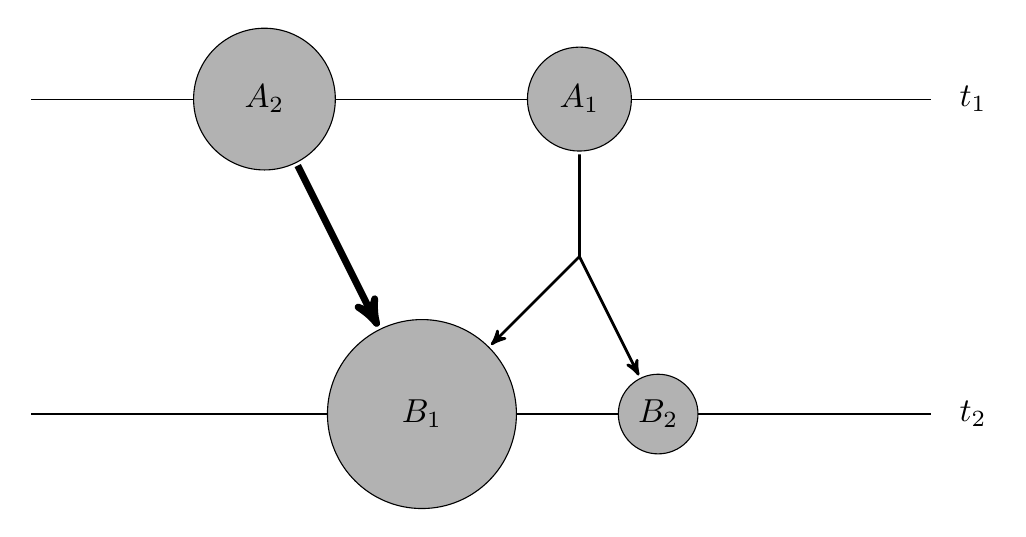
\begin{tikzpicture}[xscale=1,yscale=1,samples=400, transform shape,every node/.style={scale=1.2}, shorten <=1pt, shorten >=1pt]


        %===========================
        % Timelines
        %===========================
        
        \draw (5,0) -- (16.5, 0);
        \draw (5,4) -- (16.5, 4);
        \node at (17,4) {$t_1$};
        \node at (17,0) {$t_2$};
        
        
        
        %===========================
        % Haloes
        %===========================        
        \draw node (A1) at (10,0) [fill=gray!60,circle,minimum size=2.0cm, draw]{$B_1$};
        \draw node (A2) at (13,0) [fill=gray!60,circle,minimum size=0.4cm, draw]{$B_2$};
        \draw node (P) [inner sep=0,minimum size=0.01,fill=black,circle,draw] at (12,2) {};        
        
        % Left Side
        \draw node (B1) at (8,4) [fill=gray!60,circle,minimum size=1.5cm, draw]{$A_2$}; 
        \draw[-stealth', line width=2.5pt] (B1) to (A1);      
       
        % Right Side    
        \draw node (B2) at (12,4) [fill=gray!60,circle,minimum size=1.1cm, draw]{$A_1$};
        \draw[shorten >=-1pt, line width=1pt] (B2) to (P);
        \draw[-stealth', shorten <=0pt, line width=1pt] (P) to (A1);
        \draw[-stealth', shorten <=0pt, line width=1pt] (P) to (A2);
                
    \end{tikzpicture}
\end{document}